\section{Foglio esame Ale}
\pagebreak

\titleformat*{\subsection}{\fontsize{10}{12} \bfseries}
\titleformat*{\subsubsection}{\fontsize{8}{12} \bfseries}

\fontsize{8}{12}\selectfont

\newgeometry{left=0.5cm,right=0.5cm,top=0.5cm,bottom=0.5cm}
\begin{multicols}{2}

\subsection*{Programmazione lineare e modellazione}
\begin{enumerate}
    \item Cosa devo decidere;
    \item Quale è l'obiettivo;
    \item Come sono caratterizzate le soluzioni ammissibili(Vincoli del problema);
    \item Specificare il valore delle variabili.
\end{enumerate}
Se aggiungo variabili logiche si attivano con $x_i <= M y_i$.

$M$ è grande come il massimo raggiungibile dalla $x_i$ oppure dalla somma delle $X$ se queste sono attivate assieme.

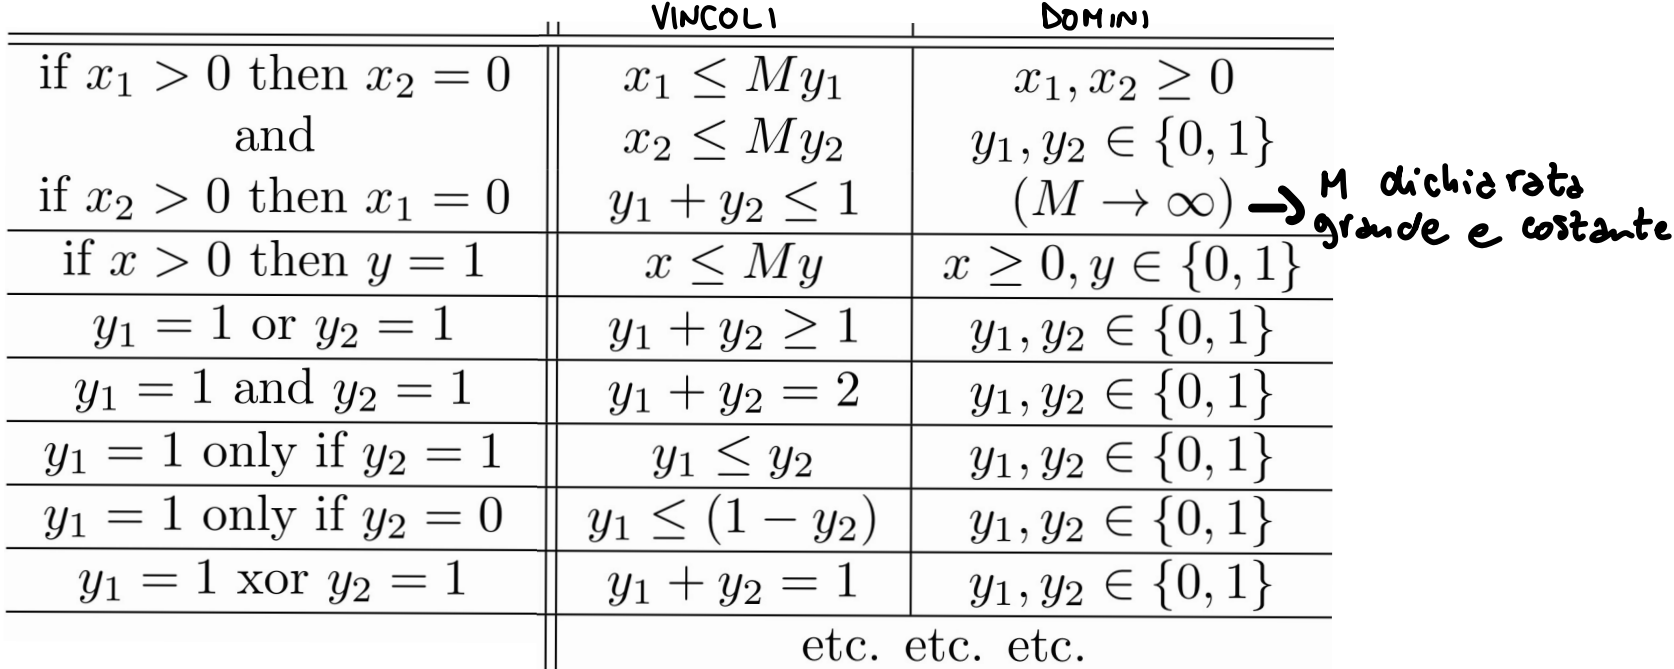
\includegraphics[width=0.9\linewidth]{img/vincoli_pl.png}

\begin{itemize}
    \item Linearità;
    \item Valori spuri;
\end{itemize}

\subsection*{Simplesso}
Convergenza in al più $\binom{n}{m}$ iterazioni;

Forma standard


\subsection*{Problemi di CCPD}
\begin{enumerate}
    \item Verifico l'ammissibilità del problema primale;
    \item Costruisco il problema duale con le relative regole;
    \item Costruisco usando l'enunciato di CCPD il problema duale;
    \item Metto a sistema le condizioni valide e ricavo gli $u_i$;
    \item Verifico l'ammissibilità del problema duale;
    \item Traggo le conclusioni.
    
    \fontsize{6}{12}\selectfont
    $
    \begin{rcases}
    x & \textrm{è ammissibile primale(verifica 1)}\\
    u & \textrm{è ammissibile duale(verifica 5)}\\
    x,u & \textrm{sono in scarti complementari(costruzione 3)}
    \end{rcases} 
    \Rightarrow
    x,u \quad \textrm{sono ottime}      
    $
    \fontsize{8}{12}\selectfont

    \item Posso verificare che $z,w$ ottime sono coincidenti.
\end{enumerate}

\subsection*{Regole di trasformazione CCPD}
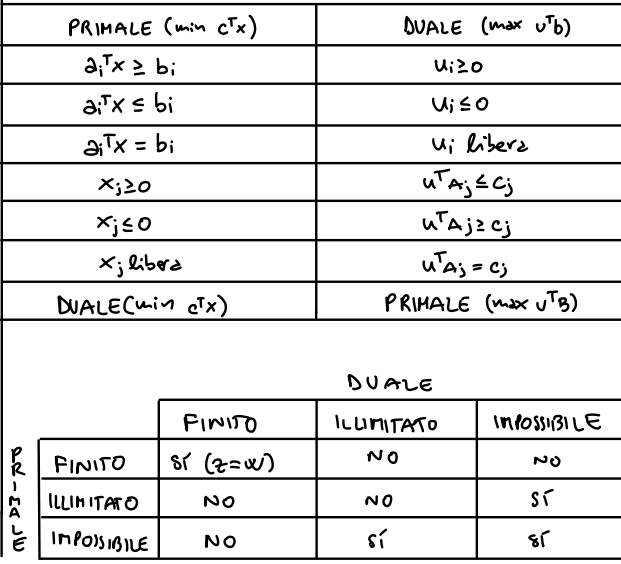
\includegraphics[width=0.9\linewidth]{img/trasformazioneCCPD.png}
\subsection*{Branch and bound}
\subsubsection*{Problemi di minimo}
\subsubsection*{Problemi di massimo}


\end{multicols}
\restoregeometry